%%%%%%%%%%%%%%%%%%%%%%%%%%%%%%%%%%%%%%%%%%%%%%%%%%%%%%%%%%%%
%% Chapter 5 — Learned Models and Online Adaptation (14–22 pages)
%% Purpose: develop the learned actuator representations,
%% explain their training objectives, and establish the
%% distinction between robust modeling and explicit online
%% adaptation.
%%%%%%%%%%%%%%%%%%%%%%%%%%%%%%%%%%%%%%%%%%%%%%%%%%%%%%%%%%%%
\chapter{Learned Models and Online Adaptation}
\label{chap:models}

The previous chapter established how the Simscape datasets were generated and
why both closed-loop operation and open-loop valve excitation were required.
This chapter develops the learned actuator representations that consume those
datasets: the inverse-dynamics (ID) and forward-dynamics (FD) networks that
form the PPO1 actuator path, and the command-conditioned reduced-order model
(ROM) that replaces them in the PPO2 path. Each model is presented with its
exact input--output contract, architecture, training objective, and offline
validation evidence, because a recurring result of this work is that standard
supervised scores alone were not sufficient to accept any of these models: a
forward model can achieve near-perfect one-step $R^2$ while having learned
almost nothing about valve authority
(Section~\ref{sec:models:fd}). All models are trained on cylinder-space
signals only; the mapping between cylinder space and task space is handled by
the kinematic layers of Chapter~\ref{chap:system} and the control integration
is described in Chapter~\ref{chap:control}.

\section{Modeling Overview and Common Notation}
\label{sec:models:overview}

\subsection{Cylinder-space signals}

All learned models in this thesis operate on the four hydraulic cylinders of
the MULAG arm, indexed $i \in \{1,\dots,4\}$ in the fixed order slew cylinder
(\emph{Drehzapfen}), boom cylinder~I (\emph{Ausleger~I}), boom cylinder~II
(\emph{Ausleger~II}), and head pivot cylinder (\emph{Messerkopf-Schwenk}).
The passive fifth joint is not actuated and does not appear in any model
input. At the learned-model sample time $T = \unit[0.05]{s}$, the discrete
time index $k$ refers to the cylinder-space state
%
\begin{equation}
  \label{eq:models:state}
  \bm{x}_k \in \mathbb{R}^4, \qquad
  \dot{\bm{x}}_k \in \mathbb{R}^4, \qquad
  \Delta\bm{p}_k \in \mathbb{R}^4, \qquad
  \bm{F}_k \in \mathbb{R}^4,
\end{equation}
%
where $\bm{x}$ collects the cylinder extensions in meters, $\dot{\bm{x}}$ the
extension velocities, $\Delta\bm{p}$ the chamber pressure differences, and
$\bm{F}$ the logged rod forces. The valve command vector
$\bm{u}_k \in [-1,1]^4$ is the normalized spool command of the four
proportional valves. Desired quantities carry a star; the desired cylinder
command produced by the task controller is the pair
%
\begin{equation}
  \label{eq:models:command}
  \bm{c}_k = \bigl[\Delta\bm{x}^{*}_k,\; \Delta\dot{\bm{x}}^{*}_k\bigr]
  \in \mathbb{R}^{8},
\end{equation}
%
i.e.\ the extension increment and the extension-velocity increment that the
controller wants to realize over the next sample. Predictions of a model
carry a hat. Table~\ref{tab:models:notation} summarizes the notation used
throughout this chapter.

\begin{table}[tb]
  \centering
  \caption{Cylinder-space notation used by all learned models.}
  \label{tab:models:notation}
  \begin{tabular}{llp{7.6cm}}
    \toprule
    Symbol & Dimension & Meaning \\
    \midrule
    $T$ & -- & learned-model sample time, $\unit[0.05]{s}$ \\
    $\bm{x}_k$, $\dot{\bm{x}}_k$ & $\mathbb{R}^4$ & cylinder extension [m] and extension velocity [m/s] \\
    $\Delta\bm{p}_k$ & $\mathbb{R}^4$ & chamber pressure difference [Pa] \\
    $\bm{F}_k$ & $\mathbb{R}^4$ & logged rod force [N] \\
    $\bm{u}_k$ & $[-1,1]^4$ & normalized proportional-valve command \\
    $\bm{c}_k = [\Delta\bm{x}^*_k, \Delta\dot{\bm{x}}^*_k]$ & $\mathbb{R}^8$ & desired extension and velocity increments \\
    $\Delta(\cdot)_k = (\cdot)_{k+1} - (\cdot)_k$ & -- & within-run one-step increment \\
    $\hat{(\cdot)}$ & -- & model prediction \\
    $\bm{h}_k$ & $\mathbb{R}^{128}$ & recurrent latent state of the ROM encoder \\
    \bottomrule
  \end{tabular}
\end{table}

\subsection{Two actuator representations, one contract}

Figure~\ref{fig:models:overview} shows the two learned actuator paths side by
side. In the PPO1 path, actuation is represented by two separate networks:
the ID network maps the current hydraulic state and a desired increment to a
valve command, and the FD network maps a valve command and the current state
to the predicted state increment. Their composition
$f_{\mathrm{FD}} \circ f_{\mathrm{ID}}$ predicts what a commanded increment
will actually do to the cylinders. In the PPO2 path, one command-conditioned
ROM replaces this composition: it receives the same desired command
$\bm{c}_k$, predicts the valve internally, and propagates pressure, velocity,
and extension through an explicit, physically structured update
(Section~\ref{sec:models:rom}). Both paths terminate in the same bounded
PhysX cylinder position target inside the IsaacLab
environment~\cite{mittal2023orbit}, and both are driven by the same
damped-least-squares task controller and residual PPO
policy~\cite{schulman2017proximal,johannink2019residual} described in
Chapter~\ref{chap:control}. The experimental variable between PPO1 and PPO2
is therefore the actuator representation alone.

\begin{figure}[tb]
  \centering
  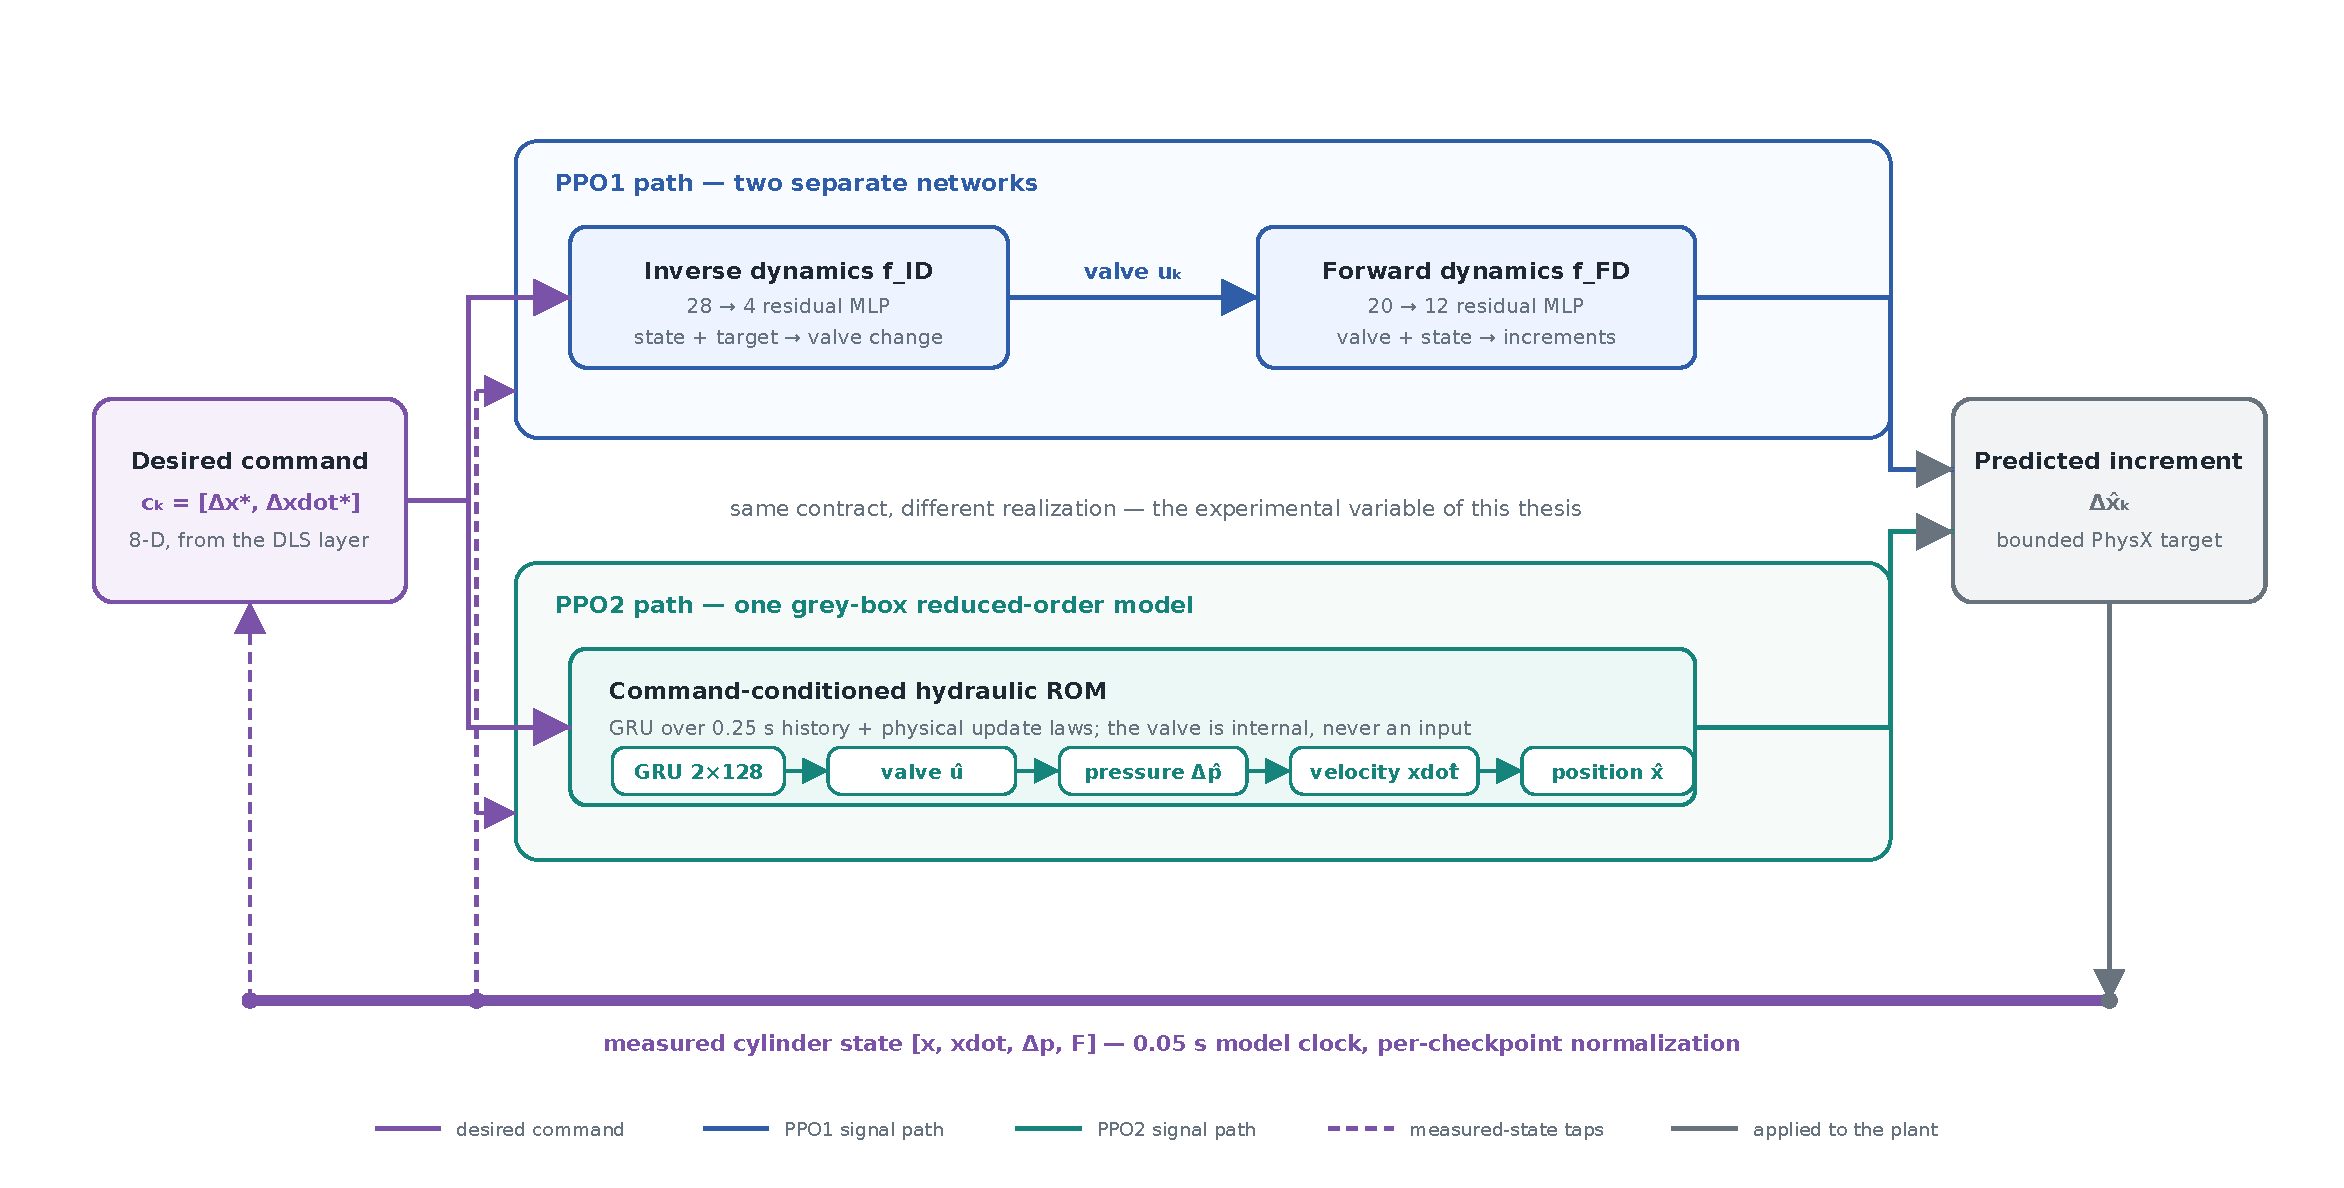
\includegraphics[width=\textwidth]{images/models_overview}
  \caption{The two learned actuator representations as parallel lanes
  around one shared contract. Both consume the same desired cylinder
  command and the same measured cylinder state from the feedback bus,
  and both produce the predicted increment that becomes the bounded
  PhysX target. The PPO1 lane composes two separately trained networks;
  the PPO2 lane realizes the command inside a single grey-box model
  whose valve signal is internal. Training-time data flow is described
  in Chapter~\ref{chap:data}.}
  \label{fig:models:overview}
\end{figure}

\subsection{Common conventions}

Three conventions apply to every model in this chapter.

\paragraph{Increment targets.}
All dynamic targets are within-run one-step increments,
$\Delta \bm{x}_k = \bm{x}_{k+1} - \bm{x}_k$, never absolute states. This
removes the dominant static component of the signals and makes the
persistence solution ($\Delta\hat{\bm{x}} = \bm{0}$) an explicit, testable
baseline rather than a hidden local minimum.

\paragraph{Per-checkpoint normalization.}
Every checkpoint stores the mean $\bm{\mu}$ and standard deviation
$\bm{\sigma}$ of its own training inputs and targets, and inference
normalizes each feature as
%
\begin{equation}
  \label{eq:models:norm}
  \tilde{\xi} = \frac{\xi - \mu_\xi}{\sigma_\xi}.
\end{equation}
%
Statistics are never shared between checkpoints; mixing the statistics of two
checkpoints silently invalidates any comparison between them, so the loader
enforces the stored contract.

\paragraph{Causal timing.}
Model inputs at step $k$ contain only quantities available at step $k$
(including the previously applied command), and targets are the measured
transition to step $k+1$. During dataset construction this alignment is
checked explicitly against the within-run differences of the logged states
(Chapter~\ref{chap:data}).

\paragraph{Gate-based acceptance.}
Finally, no model in this thesis is promoted on a supervised score.
Every candidate passes the fixed gate sequence of
Figure~\ref{fig:models:acceptance}: offline accuracy, input-ablation
authority, in-simulator cylinder gates, and the task-space tracking
gate, in that order. Each ``no'' exit names the repair that experience
showed to be the right one, and the promoted checkpoints are recorded
with their hashes for provenance. The sections that follow report, for
each model, exactly where in this ladder it initially failed and what
fixed it.

\begin{figure}[tb]
  \centering
  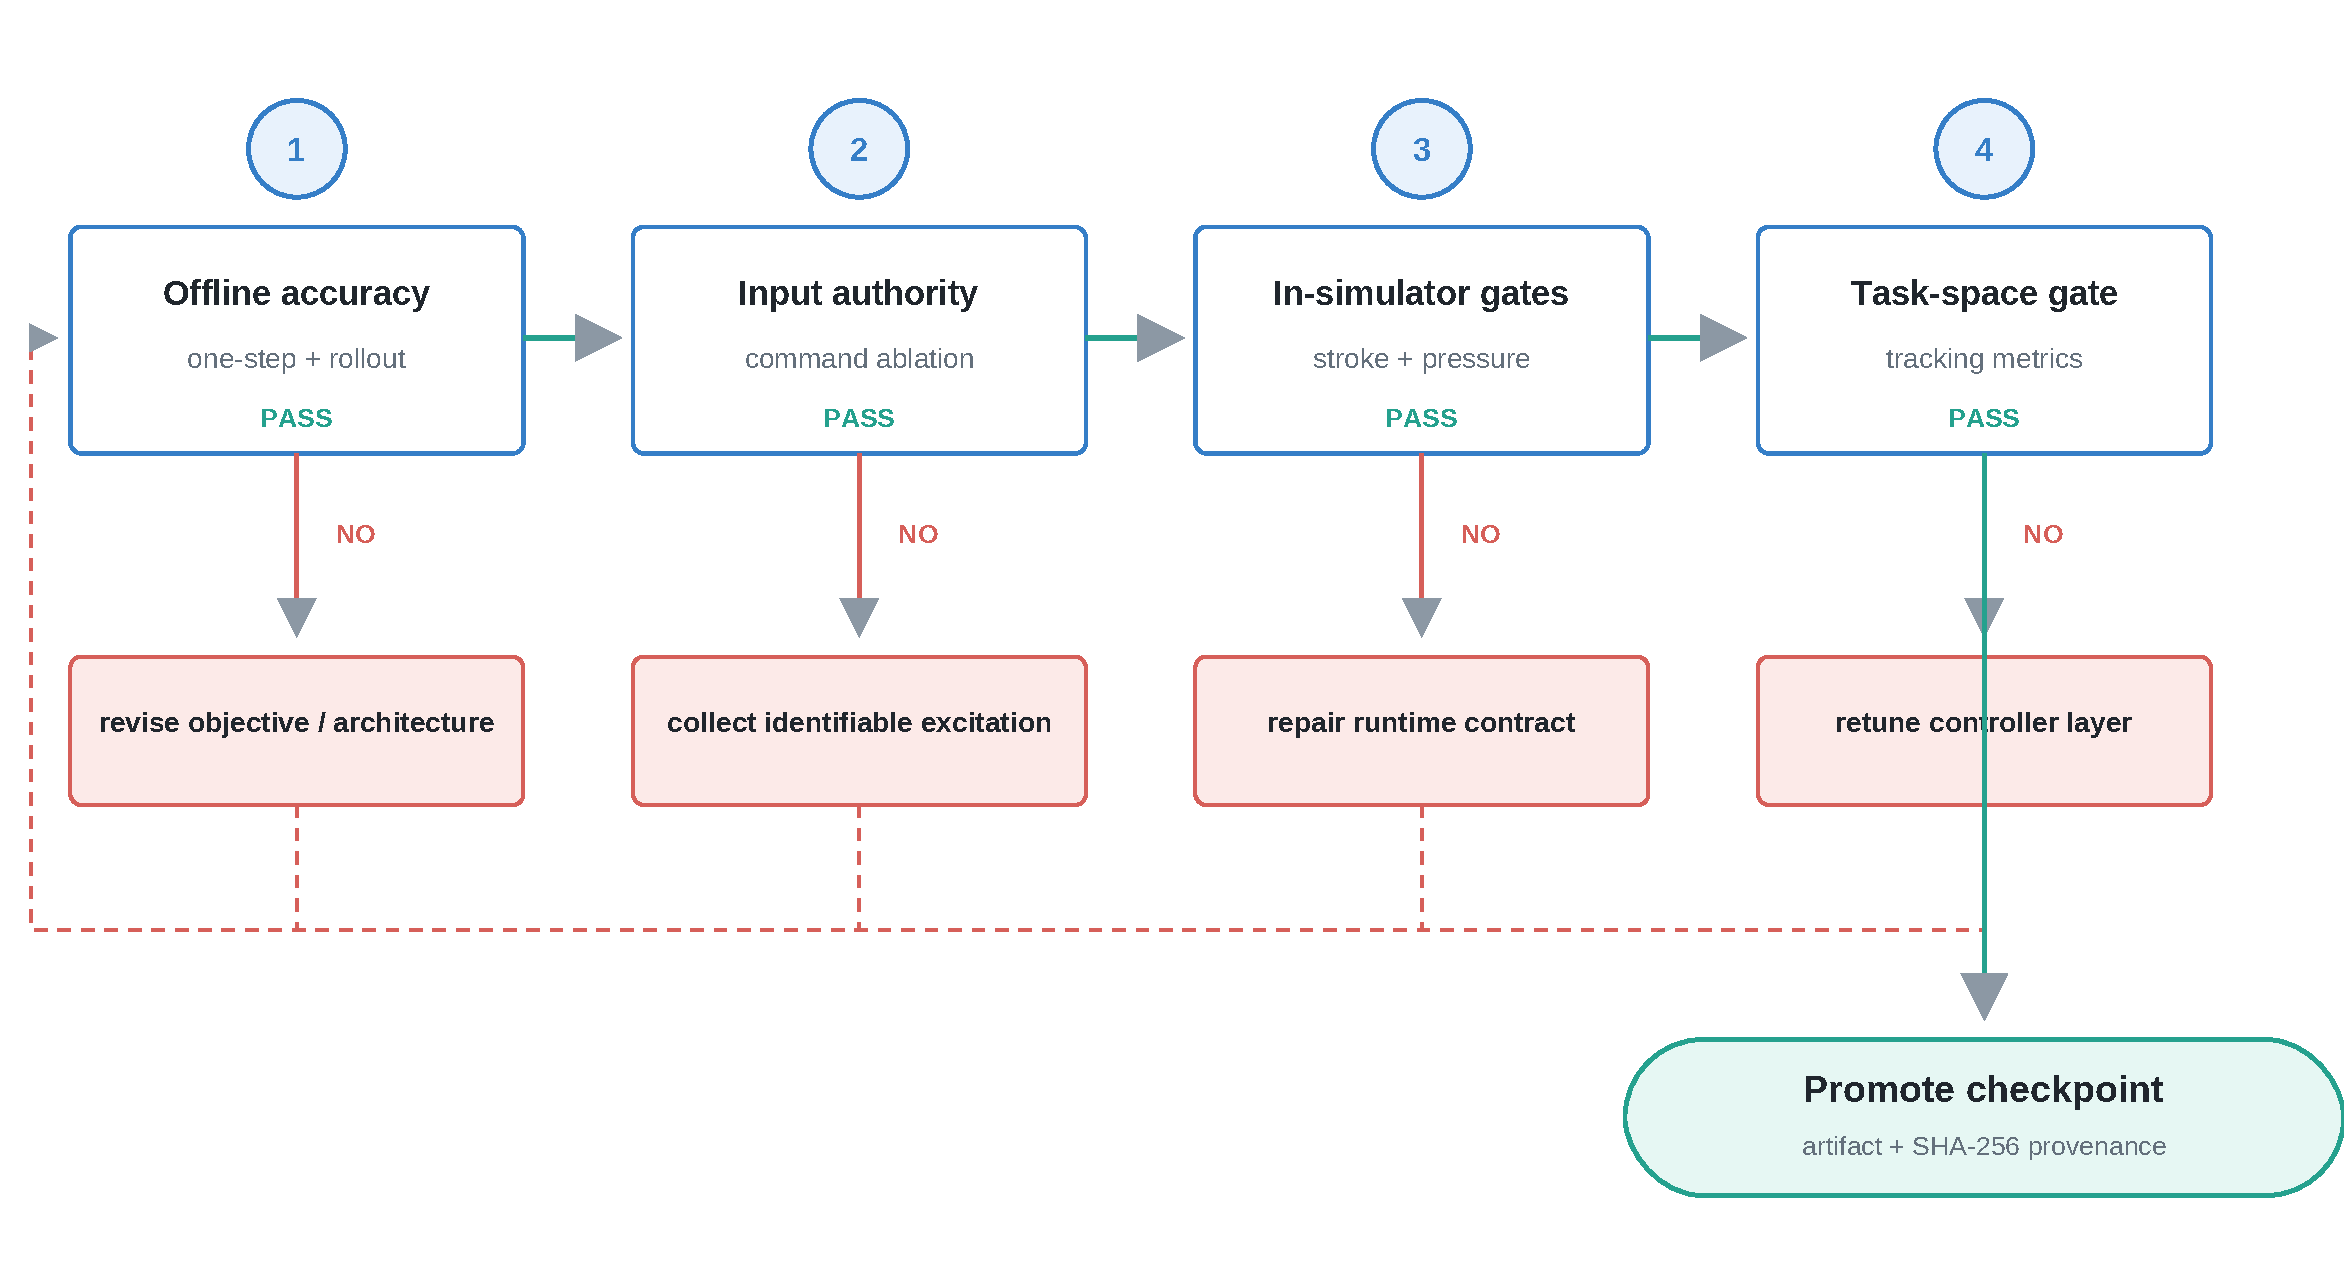
\includegraphics[width=.8\textwidth]{images/models_acceptance_flow}
  \caption{The acceptance ladder that every learned model in this
  thesis must climb before deployment. A candidate that fails a gate
  exits right into the corresponding repair loop and re-enters from the
  top; only a candidate that passes all four gates is promoted, and the
  promoted artifact is recorded together with its SHA-256 hash.}
  \label{fig:models:acceptance}
\end{figure}

\subsection{Data provenance in brief}

Two dataset families from Chapter~\ref{chap:data} are consumed here. The
\emph{closed-loop} family consists of the aligned Simscape
exports~\cite{mathworks2024simscape} used for supervised ID and FD training
and, after exact run-and-timestamp alignment, for the command-ROM dataset:
$452\,400$ transitions at $T=\unit[0.05]{s}$ from $1\,040$ runs, split by
complete runs into $936$ training, $52$ validation, and $52$ test runs
($407\,160$ / $22\,620$ / $22\,620$ samples). The \emph{open-loop} family is
the strict valve-excitation export used to repair the FD model: four $64$-s
runs sampled at $\unit[0.01]{s}$, in which the same rank-4 multi-input
open-loop excitation is applied to four distinct plant draws
(nominal, randomized hydraulics, randomized mechanics, both). Its properties
and the reasons it was necessary are analyzed in
Section~\ref{sec:models:fd}.

\section{Inverse Dynamics Model}
\label{sec:models:id}

\subsection{Input--output contract}

The ID network answers the question the low-level controller actually asks:
\emph{given the current hydraulic state, which valve command realizes a
desired cylinder increment?} Its contract is
%
\begin{equation}
  \label{eq:models:id-contract}
  \Delta\bm{u}_k = f_{\mathrm{ID}}
  \bigl(\bm{x}_k,\, \dot{\bm{x}}_k,\, \Delta\bm{p}_k,\, \bm{F}_k,\,
        \Delta\bm{x}^{*}_k,\, \Delta\dot{\bm{x}}^{*}_k,\, \bm{u}_{k-1}\bigr)
  \in \mathbb{R}^4 ,
\end{equation}
%
a 28-dimensional input mapped to a valve-command \emph{change}. The deployed
command is the accumulated
%
\begin{equation}
  \label{eq:models:id-apply}
  \bm{u}_k = \operatorname{clip}\bigl(\bm{u}_{k-1} + \Delta\bm{u}_k,\;
  -\bm{u}_{\max},\, \bm{u}_{\max}\bigr),
  \qquad \bm{u}_{\max} = [0.95,\, 0.95,\, 0.8,\, 0.8],
\end{equation}
%
where the per-axis limits are stored in the checkpoint. Predicting the
command change rather than the absolute command conditions the problem on the
previous operating point of the valve, which matters because proportional
valves are direction- and history-dependent around their dead zone
(Section~\ref{sec:fund:actuation-chain}). The desired increments
$\Delta\bm{x}^{*}, \Delta\dot{\bm{x}}^{*}$ in the training data are the
\emph{achieved} transitions of the logged Simscape runs, used as a proxy for
desired motion because no independent cylinder-space reference was logged;
the consequences of this proxy are examined below.

\subsection{Architecture and supervised training}

$f_{\mathrm{ID}}$ is a multilayer perceptron with an input projection to
width 512 followed by four residual blocks~\cite{he2016deep} with SiLU
activations~\cite{elfwing2018sigmoid}, layer
normalization~\cite{ba2016layer}, and dropout of
$0.02$~\cite{srivastava2014dropout}, implemented in
PyTorch~\cite{paszke2019pytorch};
Figure~\ref{fig:models:nn-architectures}(a) shows the trunk, which the
FD network shares, and Figure~\ref{fig:models:nn-architectures}(b) the
recurrent encoder that the ROM uses instead
(Section~\ref{sec:models:rom}).

\begin{figure}[tb]
  \centering
  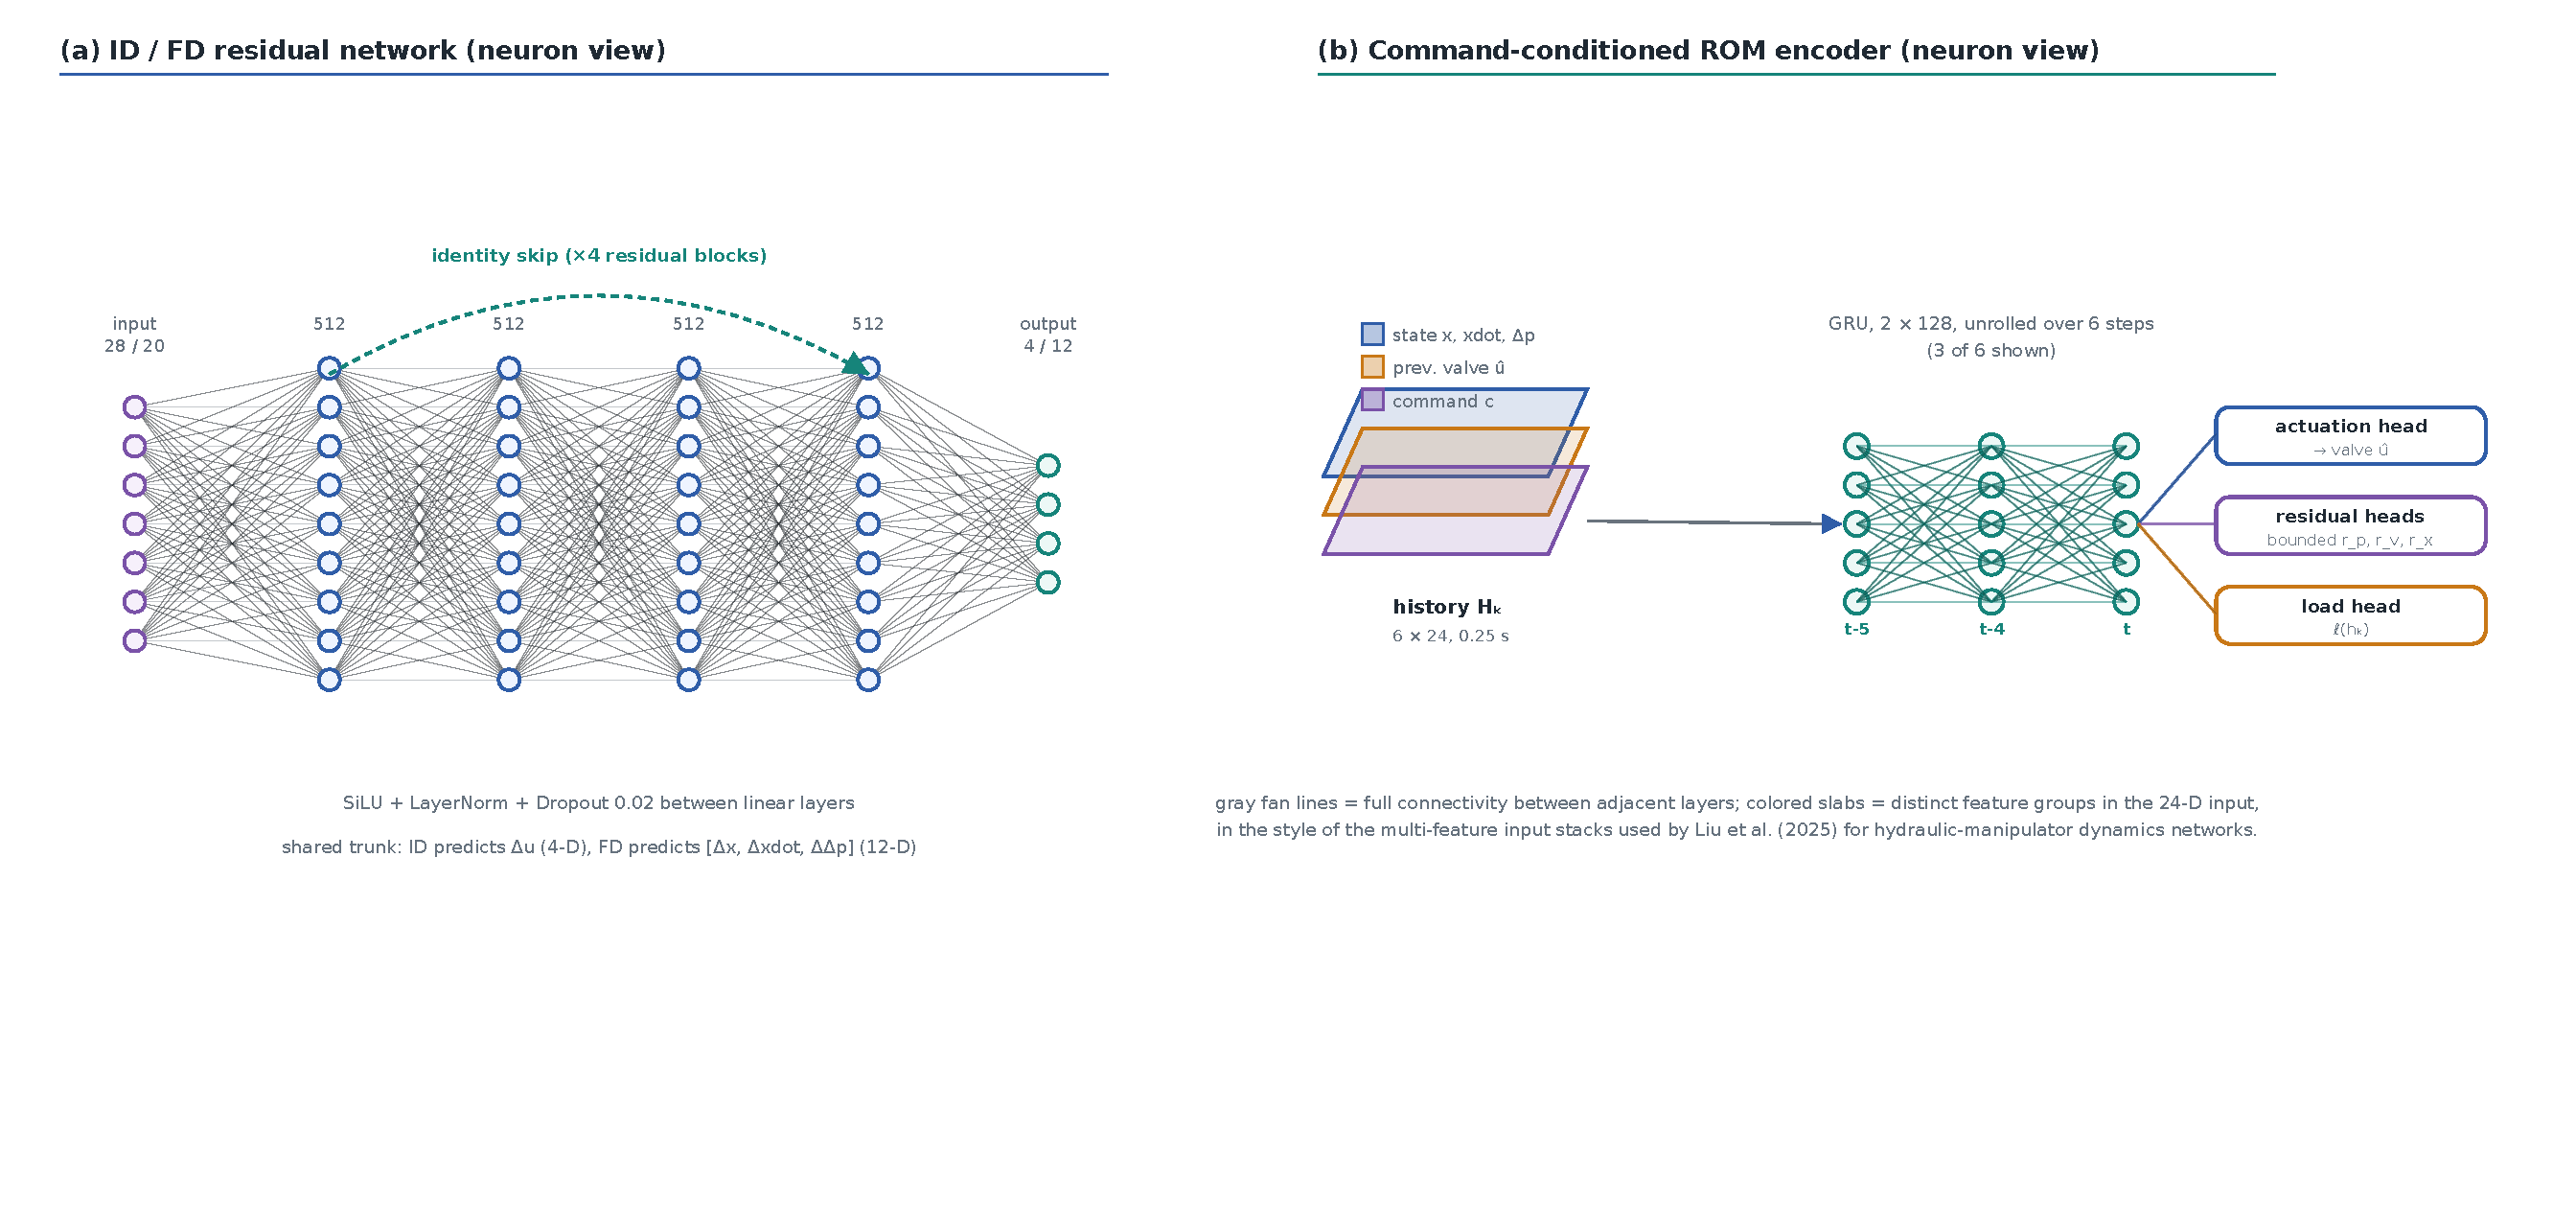
\includegraphics[width=\textwidth]{images/models_nn_architectures}
  \caption{The two network families used by the learned actuator
  models. (a)~The residual MLP trunk shared by the ID and FD networks:
  an input projection to width 512, four pre-activation residual blocks
  (Linear--LayerNorm--SiLU--Dropout--Linear with an identity skip), and
  a linear output head; only the input and output widths differ between
  ID and FD. (b)~The ROM's recurrent encoder, unrolled over its six
  history steps: each step consumes the 24-D feature vector, the hidden
  state carries pressure and command transients across time, and the
  final latent $\bm{h}_k$ feeds the actuation, residual, and load
  heads.}
  \label{fig:models:nn-architectures}
\end{figure} Training minimized the smooth-$L_1$ (Huber)
loss~\cite{huber1964robust} with transition point $\beta=0.5$ on normalized
targets using Adam~\cite{kingma2015adam} with learning rate $10^{-3}$, weight
decay $10^{-4}$, batch size $8\,192$, gradient-norm clipping at $10$, and
early stopping with patience $45$; samples in valve saturation were
up-weighted by a factor $1.25$ so that the rare saturated regime is not
ignored. The promoted checkpoint (seed 42) was selected at epoch 120 of at
most 300 with a validation loss of $0.0336$.

The supervised result was, on its face, excellent: per-valve validation
$R^2$ of $0.9996$, $0.9973$, $0.9981$, and $0.9974$. It must be stated
clearly what this number does and does not mean. It means the network
reproduces the logged valve commands from the logged states and achieved
transitions. It does not mean the composite map
$f_{\mathrm{FD}} \circ f_{\mathrm{ID}}$ has authority over the plant: since
the achieved transitions in closed-loop data are themselves produced by the
logged commands, a model can score highly by exploiting this correlation
without ever being asked to \emph{cause} a transition that was not already in
the data (Section~\ref{sec:fund:identifiability}).

\subsection{Paired control fine-tuning}
\label{sec:models:id-paired}

This deficiency became measurable when the ID and FD networks were composed.
For control, the relevant object is the \emph{paired differential response}:
the difference between what the FD predicts under the ID's command for the
actual target and under the ID's command for a zero target,
%
\begin{align}
  \bm{u}^{\mathrm{tgt}}_k &= f_{\mathrm{ID}}(\cdot,\, \bm{c}_k,\, \bm{u}_{k-1}),
  \qquad
  \bm{u}^{0}_k = f_{\mathrm{ID}}(\cdot,\, \bm{0},\, \bm{u}_{k-1}), \notag \\
  \Delta\hat{\bm{x}}^{\mathrm{pair}}_k &=
    f_{\mathrm{FD}}\bigl(\bm{u}^{\mathrm{tgt}}_k, \cdot\bigr)
  - f_{\mathrm{FD}}\bigl(\bm{u}^{0}_k, \cdot\bigr).
  \label{eq:models:paired}
\end{align}
%
If the pipeline is to be useful, $\Delta\hat{\bm{x}}^{\mathrm{pair}}_k$ must
track the requested $\Delta\bm{x}^{*}_k$. Before fine-tuning it did not: the
normalized control error of the composite was $1.00$ --- exactly the score of
predicting nothing --- with per-axis regression slopes of at most $0.004$
(Table~\ref{tab:models:paired}). Both networks were therefore fine-tuned
jointly on the control objective
%
\begin{equation}
  \label{eq:models:paired-loss}
  \mathcal{L}_{\mathrm{ctl}} =
  \bigl\| \Delta\hat{\bm{x}}^{\mathrm{pair}}
        - \Delta\bm{x}^{*} \bigr\|^2_{\mathrm{norm}}
  \;+\; \lambda_{\mathrm{ID}}\,\mathcal{L}_{\mathrm{ID}}
  \;+\; \lambda_{\mathrm{FD}}\,\mathcal{L}_{\mathrm{FD}},
\end{equation}
%
where the supervised losses $\mathcal{L}_{\mathrm{ID}}$ and
$\mathcal{L}_{\mathrm{FD}}$ are retained to limit regression from the
original data contracts. Crucially, the target blocks
$(\Delta\bm{x}^{*}, \Delta\dot{\bm{x}}^{*})$ were shuffled across valid
states during this stage, so the networks could no longer succeed by
reconstructing the logged trajectory; they had to respond to targets that the
logged controller never issued in that state.

\begin{table}[tb]
  \centering
  \caption{Effect of paired control fine-tuning on the composite
  $f_{\mathrm{FD}} \circ f_{\mathrm{ID}}$ differential response
  \eqref{eq:models:paired}, evaluated per cylinder axis on validation data.
  Before fine-tuning, the composite had essentially no control authority
  despite near-perfect supervised scores of both networks; the composite
  normalized control MSE fell from $1.0011$ to $0.1086$.}
  \label{tab:models:paired}
  \begin{tabular}{lcccc}
    \toprule
    & \multicolumn{2}{c}{Regression slope}
    & \multicolumn{2}{c}{Correlation} \\
    \cmidrule(lr){2-3} \cmidrule(lr){4-5}
    Cylinder axis & before & after & before & after \\
    \midrule
    1 (slew)      & $0.003$ & $0.818$ & $0.135$ & $0.920$ \\
    2 (boom I)    & $0.002$ & $0.928$ & $0.090$ & $0.967$ \\
    3 (boom II)   & $0.001$ & $0.849$ & $0.037$ & $0.933$ \\
    4 (head pivot)& $0.004$ & $0.912$ & $0.249$ & $0.958$ \\
    \bottomrule
  \end{tabular}
\end{table}

After 30 epochs of paired tuning the composite control MSE dropped to
$0.109$ and all four axes reached slopes above $0.8$ and correlations above
$0.92$. The resulting ID checkpoint
(\texttt{best\_id\_cylinder\_control.pt}) is the ID model deployed in all
PPO1 experiments. The fine-tuned FD from this stage, in contrast, was
accepted only as an intermediate: its remaining weakness under genuinely
independent valve excitation is the subject of the next section.

\section{Forward Dynamics Model}
\label{sec:models:fd}

\subsection{Input--output contract and supervised baseline}

The FD network predicts the one-step cylinder response to a valve command,
%
\begin{equation}
  \label{eq:models:fd-contract}
  \bigl[\Delta\hat{\bm{x}}_k,\; \Delta\hat{\dot{\bm{x}}}_k,\;
        \Delta\widehat{\Delta\bm{p}}_k\bigr]
  = f_{\mathrm{FD}}\bigl(\bm{u}_k,\, \bm{x}_k,\, \dot{\bm{x}}_k,\,
    \Delta\bm{p}_k,\, \bm{F}_k\bigr) \in \mathbb{R}^{12},
\end{equation}
%
a 20-dimensional input mapped to the three groups of state increments over
$T=\unit[0.05]{s}$. The architecture is the same residual MLP trunk as the ID
network (width 512, four residual blocks, SiLU, layer normalization, dropout
$0.02$). Supervised pretraining on the closed-loop Simscape export used
normalized MSE on all three output groups, Adam with learning rate
$10^{-4}$, weight decay $10^{-4}$, batch size $8\,192$, and an auxiliary
recursive rollout loss (weight $0.25$, horizons of 2, 5, 10, and 20 steps),
with the checkpoint selected by validation rollout
loss~\cite{nagabandi2018neural}. The selected model (epoch 291) reached
grouped one-step $R^2$ near $0.999$ for the extension increments.

\subsection{Why the supervised score was not believed}
\label{sec:models:fd-identifiability}

A model intended to give a policy gradient information about actuation must
respond to the \emph{valve}, not merely to the state history. This property
was tested directly with an input ablation: zeroing the valve input of the
pretrained FD barely changed its long-horizon rollout error
(valve-zero error ratio $\approx 0.94$ at a $\unit[0.5]{s}$ horizon;
Figure~\ref{fig:models:fd-authority}, dashed orange versus solid orange).
The model had learned to extrapolate the smooth kinematics of closed-loop
operation --- effectively a sophisticated persistence model --- because in
feedback data the controller makes valve command and state history nearly
redundant, the identifiability trap of
Section~\ref{sec:fund:identifiability}. Ablation
studies on the source MAT exports (Chapter~\ref{chap:data}) confirmed that
the valve signal was not causally identifiable from the closed-loop
distribution at all. No amount of retraining on the same distribution could
fix this; the data had to change.

\subsection{Strict open-loop excitation dataset}
\label{sec:models:fd-strict}

The repair dataset is the strict open-loop excitation export shown in
Figure~\ref{fig:models:excitation}. All four valves receive a rank-4
multi-input open-loop sequence built from long, full-authority command
plateaus: the first four segments excite one cylinder at a time, and the
final segment drives all four channels simultaneously
(Section~\ref{sec:data:open-loop}). The same excitation is applied to
four distinct plant draws --- nominal, randomized hydraulics, randomized
mechanics, and both randomized --- giving four $64$-s runs at
$\unit[0.01]{s}$ ($6\,400$ samples each, 49 logged columns). Dataset
validation established the properties that the closed-loop export lacked:
all four state trajectories are distinct; every logged target increment
agrees with the within-run difference $\bm{x}_{k+1}-\bm{x}_k$; valve history
alone predicts the pressure response with $R^2 \approx 0.80$--$0.85$; the
valve regressors have variance-inflation factors of only 7--10; and
pressure-relief saturation occupies 9--22\,\% of the samples, so the
saturated regime is represented but not dominant. An earlier excitation
export was rejected outright because half of its runs duplicated state
trajectories and the valve was again not causally identifiable --- a reminder
that excitation data must itself be audited, not assumed
informative~\cite{isermann2011identification}.

\begin{figure}[tb]
  \centering
  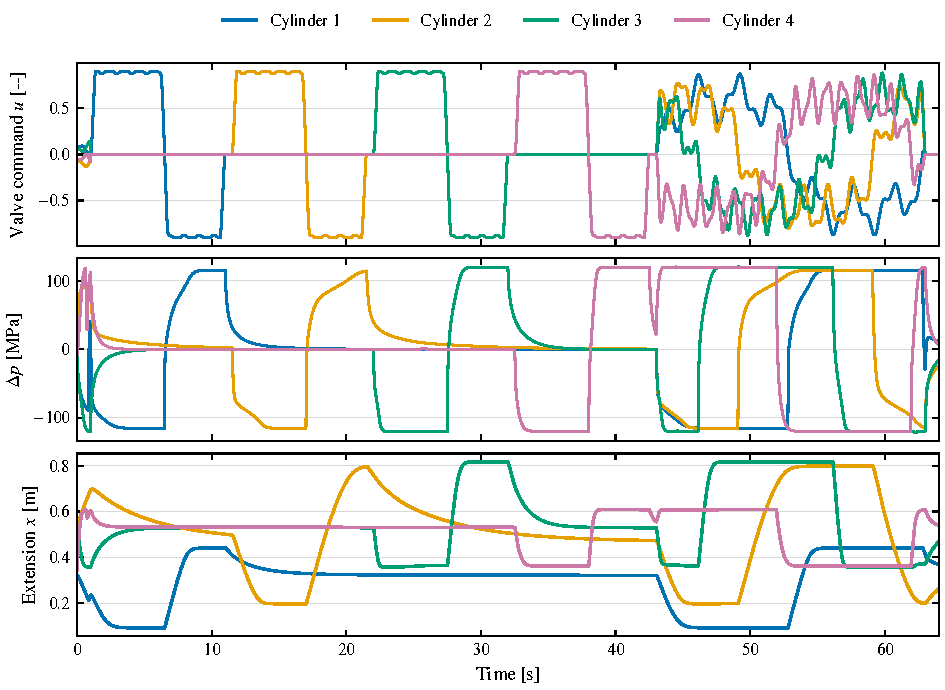
\includegraphics[width=\textwidth]{images/ch5_excitation_dataset}
  \caption{One run of the strict open-loop excitation dataset (nominal plant
  draw, $\unit[0.01]{s}$ sampling). Top: the rank-4 open-loop valve
  commands; the channels are excited individually in the first four segments
  and simultaneously in the final segment. Middle: resulting chamber
  pressure differences, including relief-limit episodes. Bottom: cylinder
  extension responses. The same excitation is repeated on three further
  randomized plant draws.}
  \label{fig:models:excitation}
\end{figure}

For FD training, five consecutive $\unit[0.01]{s}$ samples are combined into
one $\unit[0.05]{s}$ transition, with the valve input taken as the command
held at the beginning of the window. Each run is divided into 20 temporal
blocks with every fifth block assigned to validation and five-sample guard
intervals removed at each boundary, so no transition window crosses a split
boundary while train and validation samples still cover comparable pose and
energy regimes. A plain last-20\,\% split was tried and rejected because it
changed the target spread between train and validation by a factor of
1.3--2.3 and would therefore have tested extrapolation to a different
operating regime rather than generalization within one.

\subsection{Strict retraining objective}

Starting from the paired-control FD checkpoint, the promoted retraining run
(150 epochs, Adam, learning rate $3\times10^{-4}$) minimized
%
\begin{equation}
  \label{eq:models:fd-strict-loss}
  \mathcal{L}_{\mathrm{FD}} =
    \mathcal{L}_{\mathrm{Huber}}^{\mathrm{strict}}
    + 0.25\, \mathcal{L}_{\mathrm{Huber}}^{\mathrm{MAT}}
    + 2.0\, \mathcal{L}_{\mathrm{roll}}^{(10)}
    + 10.0\, \mathcal{L}_{\mathrm{kin}},
\end{equation}
%
combining the one-step Huber loss on the strict data, a replay term on the
original closed-loop data (weight $0.25$, retained because ablation showed it
improves state coverage and extension accuracy), a 10-step
($\unit[0.5]{s}$) recursive rollout loss, and a
kinematic-consistency term enforcing the trapezoidal identity
%
\begin{equation}
  \label{eq:models:trapezoid}
  \Delta\bm{x}_k = T\,\dot{\bm{x}}_k
  + \tfrac{1}{2}\, T\, \Delta\dot{\bm{x}}_k ,
\end{equation}
%
which holds in the measured strict data with $R^2 = 0.994$--$0.9997$ and ties
the predicted extension and velocity increments to each other. The Huber
loss is used because rare relief events otherwise dominate a
squared-error objective. One further, initially attractive
regularizer was evaluated and deliberately rejected: anchoring the model to a
constant valve Jacobian. The measured valve authority varies by a factor of
15--75 across pressure quartiles and can change sign, so pinning a single
global gain produced a pleasing mean response while collapsing one-step
accuracy. This is consistent with the strongly operating-point-dependent
valve--flow--pressure characteristics of hydraulic servo-systems
discussed in Section~\ref{sec:fund:actuation-chain}, and it motivates
the pressure-dependent structure adopted in the ROM
(Section~\ref{sec:models:rom}).

\subsection{Validation: valve authority restored}

\begin{figure}[tb]
  \centering
  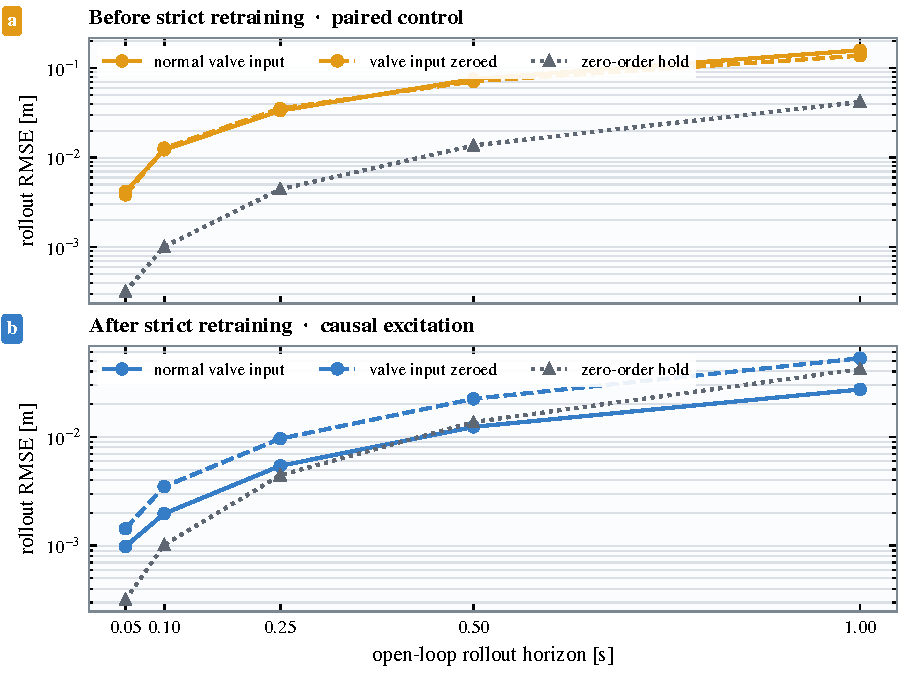
\includegraphics[width=\textwidth]{images/ch5_fd_rollout_authority}
  \caption{Open-loop extension rollout RMSE on held-out strict-excitation
  data as a function of rollout horizon, before (orange) and after (blue)
  strict retraining. Dashed curves show the same model with the valve input
  zeroed; the gap between solid and dashed is the model's usable valve
  authority. The paired-control FD is insensitive to its valve input,
  whereas the strict FD degrades by a factor of 1.8--1.9 when the valve is
  removed and outperforms the zero-order hold baseline (gray) beyond
  $\unit[0.5]{s}$.}
  \label{fig:models:fd-authority}
\end{figure}

Figure~\ref{fig:models:fd-authority} and Table~\ref{tab:models:fd-strict}
summarize the outcome. The strict FD reduces the $\unit[0.5]{s}$ extension
rollout RMSE from $\unit[75.2]{mm}$ to $\unit[12.4]{mm}$ and the
$\unit[1.0]{s}$ RMSE from $\unit[157.9]{mm}$ to $\unit[27.3]{mm}$, and ---
the decisive criterion --- its valve-zero error ratio rises from $0.94$ to
$1.81$ at $\unit[0.5]{s}$: removing the valve input now roughly doubles the
rollout error, which is exactly the sensitivity a control-relevant forward
model must exhibit. Per-axis one-step extension-increment $R^2$ improved
from the range $[-5.7,\, 0.60]$ to $[0.76,\, 0.98]$. Two honest limitations
remain. First, at very short horizons ($\leq \unit[0.25]{s}$) the zero-order
hold baseline is still competitive, because extension simply does not move
far in $\unit[0.05]{s}$; the learned model's value appears at the horizons
over which a target increment must be committed. Second, the
velocity-increment outputs remain poorly predicted (near-zero or negative
$R^2$ on two axes, dominated by relief transients that a memoryless
$\unit[0.05]{s}$ model cannot resolve). The deployed controller therefore
integrates only $\Delta\hat{\bm{x}}$, the accurately modeled and directly
validated quantity, and treats the velocity output as diagnostic.

\begin{table}[tb]
  \centering
  \caption{Strict-excitation validation of the FD model before and after
  strict retraining. The valve-zero error ratio is the rollout RMSE with
  zeroed valve input divided by the RMSE with the true valve input at a
  $\unit[0.5]{s}$ horizon; a ratio near 1 means the model ignores the valve.}
  \label{tab:models:fd-strict}
  \begin{tabular}{lcc}
    \toprule
    Metric & Paired-control FD & Strict FD \\
    \midrule
    Valve-zero error ratio at $\unit[0.5]{s}$ & $\approx 0.94$ & $1.81$ \\
    Extension rollout RMSE at $\unit[0.5]{s}$ & $\unit[75.2]{mm}$ & $\unit[12.4]{mm}$ \\
    Extension rollout RMSE at $\unit[1.0]{s}$ & $\unit[157.9]{mm}$ & $\unit[27.3]{mm}$ \\
    One-step $\Delta x$ $R^2$ (per-axis range) & $-5.7$ to $0.60$ & $0.76$ to $0.98$ \\
    \bottomrule
  \end{tabular}
\end{table}

For completeness, an intermediate rank-preserving fine-tuning stage between
the supervised and paired stages regularized the valve-to-extension
differential map with a finite-difference Jacobian penalty; the resulting
checkpoint has a full-rank (rank-4) valve Jacobian with condition number
$\approx 2.3$ and is retained as provenance, but the strict FD supersedes it
as the active model. The strict FD
(\texttt{best\_fd\_cylinder\_strict.pt}) together with the paired-control ID
constitutes the learned actuator pair of every PPO1 experiment in
Chapter~\ref{chap:evaluation}.

\section{Reduced-Order Model}
\label{sec:models:rom}

\subsection{Motivation and design position}

The PPO1 actuator path composes two separately trained networks and, as the
previous sections showed, needed three repair stages before the composition
had authority. The PPO2 path replaces the composition with a single
\emph{command-conditioned reduced-order model} that is trained end-to-end on
exactly the quantity the controller consumes: the response of the cylinders
to a desired cylinder command. Two design decisions distinguish the ROM from
a generic sequence model. First, it is \emph{grey-box}: pressure, force,
velocity, and extension are propagated through explicit physical update
equations with trainable effective parameters, and neural components only
supply what the physics cannot --- the valve realization, unmodeled load,
and bounded residual corrections~\cite{karniadakis2021physics,lutter2019deep}.
This follows the observation from Section~\ref{sec:models:fd} that valve
authority is strongly pressure-dependent: encoding the
orifice-flow--continuity structure~\cite{merritt1967hydraulic} makes that
dependence architectural rather than something to be rediscovered from data.
Second, it is \emph{recurrent}: a GRU encoder~\cite{cho2014learning} over
$0.25$~s of history replaces the memoryless state input of the FD, in the
spirit of the learned actuator networks of
Hwangbo et al.~\cite{hwangbo2019learning}, because hydraulic response
depends on recent pressure and command history that a single sample cannot
represent.

\subsection{Input--output contract}

The ROM consumes a history of $L=6$ samples ($\unit[0.25]{s}$ at
$T=\unit[0.05]{s}$) of the 24-dimensional feature vector
%
\begin{equation}
  \label{eq:models:rom-input}
  \bm{z}_k = \bigl[\bm{x}_k,\; \dot{\bm{x}}_k,\; \Delta\bm{p}_k,\;
  \hat{\bm{u}}_{k-1},\; \bm{c}_k \bigr] \in \mathbb{R}^{24},
\end{equation}
%
i.e.\ the cylinder state, the \emph{previously predicted} valve command fed
back as recurrent state, and the current desired command
$\bm{c}_k \in \mathbb{R}^8$ of \eqref{eq:models:command}. The actual valve
command appears only as a training target for the internal valve head; at
runtime no valve signal enters the model. From
$\mathcal{H}_k = (\bm{z}_{k-L+1}, \dots, \bm{z}_k)$ the ROM predicts the
internal valve realization and the full next cylinder state,
%
\begin{equation}
  \label{eq:models:rom-output}
  \bigl(\hat{\bm{u}}_k,\; \Delta\hat{\bm{p}}_k,\;
        \Delta\hat{\dot{\bm{x}}}_k,\; \Delta\hat{\bm{x}}_k\bigr)
  = f_{\mathrm{ROM}}\bigl(\mathcal{H}_k\bigr),
\end{equation}
%
which jointly replaces the ID--FD composition of the PPO1 path.

\subsection{Grey-box structure}

\begin{figure}[tb]
  \centering
  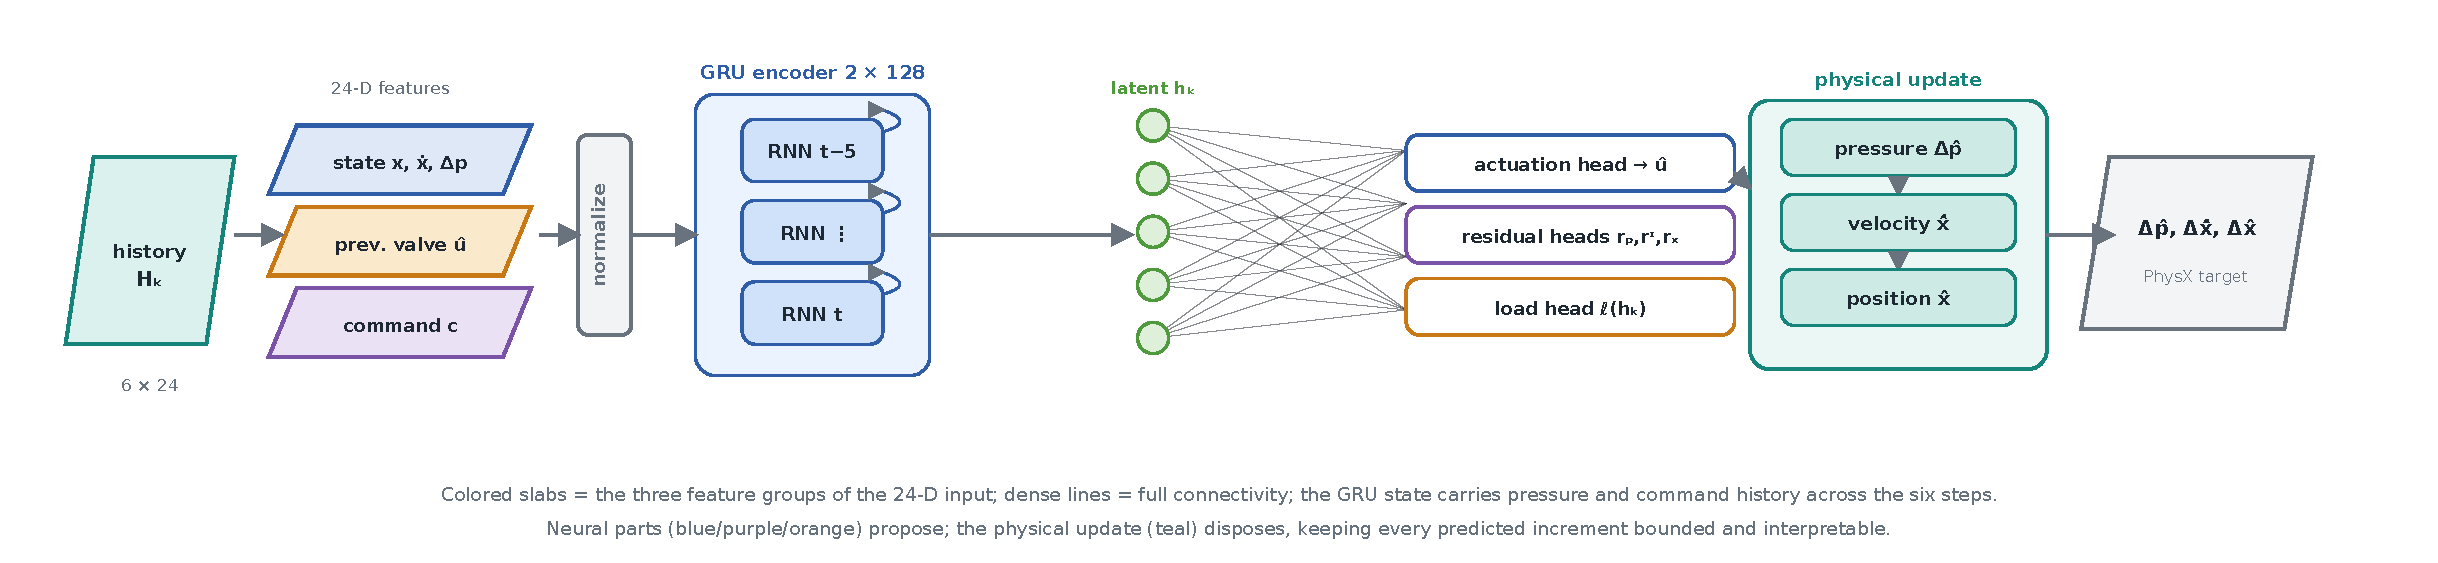
\includegraphics[width=\textwidth]{images/models_rom_pipeline}
  \caption{Structure of the command-conditioned reduced-order model as
  a data-flow pipeline. The $\unit[0.25]{s}$ history is split into its
  three feature groups (state, previously predicted valve, desired
  command), normalized, and passed through the recurrent GRU encoder
  whose hidden state carries pressure and command history across the six
  steps. The final latent feeds three fully connected heads: the
  actuation head realizes the command as an internal valve signal, the
  residual heads supply tanh-bounded corrections, and the load head the
  configuration load. The state is then propagated through the explicit
  pressure \eqref{eq:models:rom-pressure}, velocity
  \eqref{eq:models:rom-velocity}, and position
  \eqref{eq:models:rom-position} updates with trainable effective
  hydraulic parameters, so the neural parts propose and the physics
  disposes.}
  \label{fig:models:rom-structure}
\end{figure}

Figure~\ref{fig:models:rom-structure} shows the computation. The normalized
history is encoded by a two-layer GRU of width 128 (dropout $0.05$); the
final latent $\bm{h}_k$ and the command $\bm{c}_k$ feed a small actuation
head whose output passes through a learnable smooth dead-zone element ---
per-cylinder trainable width and asymmetric gains, built from softplus and
$\tanh$ primitives so it remains differentiable --- reflecting the dead band
and direction-dependent gain of proportional valves
(Section~\ref{sec:fund:actuation-chain}). The resulting
internal actuation $\hat{a}_i \in [-1,1]$ drives an orifice-flow and
continuity update per cylinder $i$,
%
\begin{align}
  q_i &= \hat{a}_i\, k_{q,i}\,
    \sqrt{\tfrac{1}{2}\bigl(p_{s,i} - \operatorname{sgn}(\hat{a}_i)\,
    \Delta p_i\bigr)_{+}}, \notag \\
  \Delta \hat{p}_{i,k+1} - \Delta p_{i,k} &=
    \frac{4\beta_i}{V_i(x_i)}
    \bigl(q_i - A_i \dot{x}_i - k_{\ell,i}\, \Delta p_i\bigr)\, T
    \;+\; r_{p,i},
  \label{eq:models:rom-pressure}
\end{align}
%
with effective bulk modulus $\beta_i$, supply pressure $p_{s,i}$, flow gain
$k_{q,i}$, leakage coefficient $k_{\ell,i}$, piston area $A_i$, and
extension-dependent chamber volume
$V_i(x_i) = V_{0,i} + A_i (x_i - x_{\mathrm{ref},i})$; the softplus-smoothed
pressure margin $(\cdot)_+$ keeps the square root differentiable near the
supply limit. The pressure then produces force, and force produces motion:
%
\begin{align}
  \hat{F}_i &= \Delta\hat{p}_{i,k+1} A_i + r_{F,i}, \qquad
  \ddot{x}_i = \frac{\hat{F}_i - c_{v,i}\,\dot{x}_i - \ell_i(\bm{h}_k)}{m_i},
  \notag \\
  \dot{\hat{x}}_{i,k+1} &= \dot{x}_{i,k}
    + \operatorname{sat}\bigl(T\,\ddot{x}_i + r_{v,i}\bigr),
  \label{eq:models:rom-velocity} \\
  \hat{x}_{i,k+1} &= x_{i,k}
    + \tfrac{T}{2}\bigl(\dot{x}_{i,k} + \dot{\hat{x}}_{i,k+1}\bigr)
    + r_{x,i},
  \label{eq:models:rom-position}
\end{align}
%
where $c_{v,i}$ is a viscous friction coefficient, $m_i$ an effective
modal mass, and $\ell_i(\bm{h}_k)$ a neural load head that captures the
configuration-dependent gravitational and coupling load. All physical
parameters are trained in log-space with hard clamps to physically plausible
ranges, so they can adapt to the data without leaving their meaning behind.
The trapezoidal position update \eqref{eq:models:rom-position} is the same
identity \eqref{eq:models:trapezoid} that the strict data satisfies almost
exactly. The neural residuals $r_{p}, r_{v}, r_{x}$ are $\tanh$-bounded to
10\,\% of the pressure step limit, 10\,\% of the velocity step limit, and
$\unit[1]{cm}$ respectively: large enough to absorb model error, too small
to let the network bypass the physics. This bounded-residual layering is
the central robustness argument of the grey-box design --- even a poorly
trained residual cannot produce an unphysical state jump.

\subsection{Dataset and training}

The command-ROM dataset joins the aligned ID and FD closed-loop exports on
exact run identifiers and time indices, yielding the $452\,400$
transitions and run-level 936/52/52 split summarized in
Section~\ref{sec:models:overview}; the logged valve commands enter only as
supervision for the internal valve head. Training (seed 17, Adam, learning
rate $3\times10^{-4}$, weight decay $10^{-5}$, batch size $2\,048$,
gradient-norm clipping at 5) follows a four-stage rollout curriculum with
horizons $H \in \{1, 5, 20, 50\}$ and stage lengths of $30/30/30/40$ epochs:
each stage optimizes the weighted one-step losses plus a recursive rollout
loss at its horizon, with scheduled sampling ramping from fully teacher-forced
to 75\,\% self-fed within each rollout~\cite{bengio2015scheduled}. The loss
weights (pressure $1.0$, velocity $2.0$, extension $1.0$, rollout $2.0$,
valve supervision $1.0$, residual penalty $0.1$, actuation regularization
$0.5$) penalize the residual heads explicitly so that explanatory burden
stays on the physical terms. The logged force channel receives zero
supervised weight: it failed a piston-area consistency audit on the current
curriculum ($F \neq \Delta p \cdot A$ within tolerance), and supervising a
head on a label that violates the model's own structure would corrupt the
pressure chain. The ROM still exposes its pressure-derived force
internally; force supervision can be enabled once a reliable chamber-force
label is available.

\begin{figure}[tb]
  \centering
  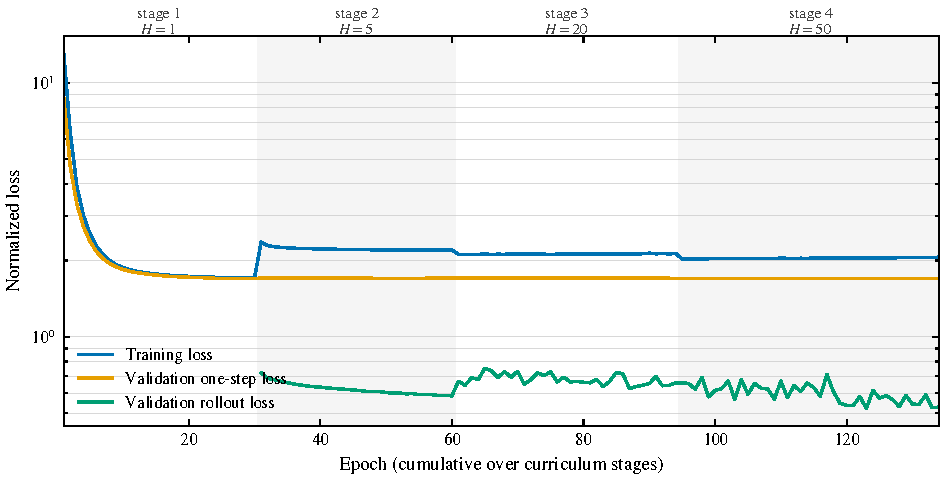
\includegraphics[width=\textwidth]{images/ch5_rom_training_history}
  \caption{Training history of the promoted command-ROM run over the
  four-stage rollout curriculum ($H$ is the recursive rollout horizon of
  each stage). The step in training loss at each stage boundary reflects
  the added longer-horizon rollout term; the validation one-step loss
  remains stable while the validation rollout loss continues to improve
  through stage~4.}
  \label{fig:models:rom-training}
\end{figure}

Figure~\ref{fig:models:rom-training} shows the resulting training history.
The characteristic step in the training loss at each stage boundary is the
newly added, harder rollout term; the important observation is that the
validation one-step loss does not degrade as longer horizons are introduced,
while the validation rollout loss improves --- the curriculum buys
long-horizon stability without sacrificing one-step accuracy.

\subsection{Offline validation}

\begin{figure}[tb]
  \centering
  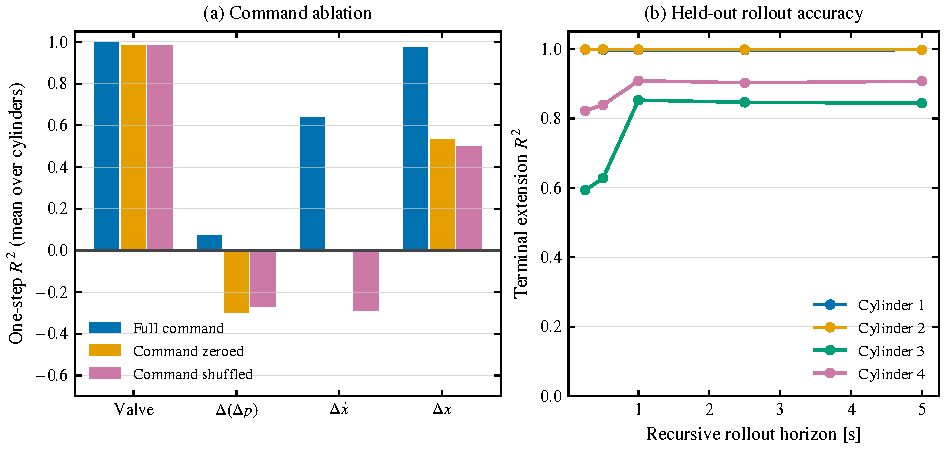
\includegraphics[width=\textwidth]{images/ch5_rom_validation}
  \caption{Offline validation of the command ROM on held-out runs.
  (a)~One-step $R^2$ per output group (mean over the four cylinders) with
  the full desired command, with the command zeroed, and with the command
  shuffled across the batch; the collapse of the velocity and extension
  scores without the true command demonstrates command authority.
  (b)~Terminal extension $R^2$ of recursive rollouts up to $\unit[5]{s}$
  (100 steps) per cylinder.}
  \label{fig:models:rom-validation}
\end{figure}

The offline acceptance report (4\,096 held-out samples, all gates passed) is
summarized in Figure~\ref{fig:models:rom-validation}. Three findings matter
for the control experiments. First, \emph{command authority}: with the true
command, mean one-step $R^2$ is $0.998$ for the internal valve prediction,
$0.64$ for the velocity increment, and $0.97$ for the extension increment;
zeroing or shuffling the command collapses the velocity score to below zero
and the extension score to $\approx 0.5$, and the $4\times4$ Jacobian of
predicted extension increment with respect to the commanded increment is
diagonally dominant with singular values $1.00$--$0.47$ and condition number
$2.14$. The model responds to what it is asked to do, per axis, which is
precisely the property whose absence broke the pretrained FD. Second,
\emph{rollout stability}: recursive rollouts remain accurate and bounded to
at least $\unit[5]{s}$ (terminal extension $R^2$ of $0.998$/$0.998$/$0.84$/
$0.91$ per cylinder), so PPO2 training rollouts do not ride on a diverging
model. Third, \emph{honest weaknesses}: the one-step pressure-increment
$R^2$ is low ($0.06$--$0.09$) --- pressure transients at $\unit[0.05]{s}$
resolution remain largely unpredictable, and the model's pressure state is
best understood as an internal latent that supports the velocity chain
rather than as a calibrated pressure estimator --- and cylinders 3 and 4
(boom~II and head pivot) are consistently harder than cylinders 1 and 2 in
both velocity and rollout scores. Inference costs $21.5\,\mu\mathrm{s}$ per
step in evaluation, which is compatible with the vectorized IsaacLab
training loop.

Beyond these aggregate scores, the acceptance protocol requires
pressure--velocity phase-plane checks, frequency-response comparisons, and
an in-simulator cylinder step gate before any PPO2 training run; a
state-only variant trained with the command zeroed throughout serves as the
mandatory comparison model for the identifiability ablations in
Chapter~\ref{chap:evaluation}. The nominal, randomized/robust, and
latent-conditioned ROM variants used in the PPO2-A/B/C experiments all share
the architecture and training protocol of this section and differ only in
their training distribution and conditioning inputs; the latent conditioning
mechanism is developed in Sections~\ref{sec:models:latent}
and~\ref{sec:models:aam}.

\section{Latent Representation of Randomized Dynamics}
\label{sec:models:latent}
% - How the teacher/encoder obtains a compact representation from
%   randomized-system context.
% - Latent dimension and training objective.
% - Latent clusters/trends vs. parameter variations — avoid
%   unsupported one-latent-one-parameter claims.
\todo{write}

\section{Arm Adaptation Module}
\label{sec:models:aam}
% - Observation history available online.
% - Temporal estimator predicting the teacher latent vector.
% - Causal deployment, update rate, warm-up history, behaviour after
%   sudden or gradual parameter changes.
\todo{write}

\section{Training and Model-Selection Protocol}
\label{sec:models:training}
% - Common train/validation/test splits.
% - Hyperparameters, early stopping, checkpoint selection, seeds.
% - Loss weighting across cylinder extension, velocity, pressure, or
%   other target groups.
\todo{write}

\section{Offline Model Evaluation}
\label{sec:models:offline-eval}
% - One-step and multi-step rollout metrics.
% - Nominal, randomized seen, unseen-parameter performance.
% - AAM latent-estimation error and adaptation delay.
% - Ablations: valve input, history length, latent conditioning,
%   dataset source.
\todo{write}
